\documentclass{article}
\usepackage{graphicx, tikz-cd} % Required for inserting images
\usepackage{amsmath, amssymb, amsthm, amsfonts, siunitx, physics}
\AtBeginDocument{\RenewCommandCopy\qty\SI}
\usepackage[version=4]{mhchem}
\usepackage[most,many,breakable]{tcolorbox}
\usepackage{geometry, xcolor, fancyhdr, varwidth}
\usepackage[Glenn]{fncychap}
%Options: Sonny, Lenny, Glenn, Conny, Rejne, Bjarne, Bjornstrup
\usepackage{hyperref, cleveref}
\usepackage{icomma, enumitem} %comma as decimal and continue enumerate with [resume]
%%%%%%%%%%%%%%%%%%%%%%%%%%%%%%
% SELF MADE COLORS
%%%%%%%%%%%%%%%%%%%%%%%%%%%%%%
\definecolor{myg}{RGB}{56, 140, 70}
\definecolor{myb}{RGB}{45, 111, 177}
\definecolor{myr}{RGB}{199, 68, 64}
\definecolor{mytheorembg}{HTML}{F2F2F9}
\definecolor{mytheoremfr}{HTML}{00007B}
\definecolor{mylenmabg}{HTML}{FFFAF8}
\definecolor{mylenmafr}{HTML}{983b0f}
\definecolor{mypropbg}{HTML}{f2fbfc}
\definecolor{mypropfr}{HTML}{191971}
\definecolor{myexamplebg}{HTML}{F2FBF8}
\definecolor{myexamplefr}{HTML}{88D6D1}
\definecolor{myexampleti}{HTML}{2A7F7F}
\definecolor{mydefinitbg}{HTML}{E5E5FF}
\definecolor{mydefinitfr}{HTML}{3F3FA3}
\definecolor{notesgreen}{RGB}{0,162,0}
\definecolor{myp}{RGB}{197, 92, 212}
\definecolor{mygr}{HTML}{2C3338}
\definecolor{myred}{RGB}{127,0,0}
\definecolor{myyellow}{RGB}{169,121,69}
\definecolor{myexercisebg}{HTML}{F2FBF8}
\definecolor{myexercisefg}{HTML}{88D6D1}
%%%%%%%%%%%%%%%%%%%%%%%%%%%%%%%%%%%%%%%%%%%%%%%%%%%%%%%%%%%%%%%%%%%%%%
% Box environments for theorems and problems
%%%%%%%%%%%%%%%%%%%%%%%%%%%%%%%%%%%%%%%%%%%%%%%%%%%%%%%%%%%%%%%%%%%%%
\setlength{\parindent}{1cm}
%================================
% Question BOX
%================================
\makeatletter
\newtcbtheorem{question}{Opgave}{enhanced,
	breakable,
	colback=white,
	colframe=myb!80!black,
	attach boxed title to top left={yshift*=-\tcboxedtitleheight},
	fonttitle=\bfseries,
	title={#2},
	boxed title size=title,
	boxed title style={%
			sharp corners,
			rounded corners=northwest,
			colback=tcbcolframe,
			boxrule=0pt,
		},
	underlay boxed title={%
			\path[fill=tcbcolframe] (title.south west)--(title.south east)
			to[out=0, in=180] ([xshift=5mm]title.east)--
			(title.center-|frame.east)
			[rounded corners=\kvtcb@arc] |-
			(frame.north) -| cycle;
		},
	#1
}{def}
\makeatother
%================================
% DEFINITION BOX
%================================

\newtcbtheorem[]{Definition}{Definition}{enhanced,
	before skip=2mm,after skip=2mm, colback=red!5,colframe=red!80!black,boxrule=0.5mm,
	attach boxed title to top left={xshift=1cm,yshift*=1mm-\tcboxedtitleheight}, varwidth boxed title*=-3cm,
	boxed title style={frame code={
					\path[fill=tcbcolback]
					([yshift=-1mm,xshift=-1mm]frame.north west)
					arc[start angle=0,end angle=180,radius=1mm]
					([yshift=-1mm,xshift=1mm]frame.north east)
					arc[start angle=180,end angle=0,radius=1mm];
					\path[left color=tcbcolback!60!black,right color=tcbcolback!60!black,
						middle color=tcbcolback!80!black]
					([xshift=-2mm]frame.north west) -- ([xshift=2mm]frame.north east)
					[rounded corners=1mm]-- ([xshift=1mm,yshift=-1mm]frame.north east)
					-- (frame.south east) -- (frame.south west)
					-- ([xshift=-1mm,yshift=-1mm]frame.north west)
					[sharp corners]-- cycle;
				},interior engine=empty,
		},
	fonttitle=\bfseries,
	title={#2},#1}{def}
\newtcbtheorem[]{definition}{Definition}{enhanced,
	before skip=2mm,after skip=2mm, colback=red!5,colframe=red!80!black,boxrule=0.5mm,
	attach boxed title to top left={xshift=1cm,yshift*=1mm-\tcboxedtitleheight}, varwidth boxed title*=-3cm,
	boxed title style={frame code={
					\path[fill=tcbcolback]
					([yshift=-1mm,xshift=-1mm]frame.north west)
					arc[start angle=0,end angle=180,radius=1mm]
					([yshift=-1mm,xshift=1mm]frame.north east)
					arc[start angle=180,end angle=0,radius=1mm];
					\path[left color=tcbcolback!60!black,right color=tcbcolback!60!black,
						middle color=tcbcolback!80!black]
					([xshift=-2mm]frame.north west) -- ([xshift=2mm]frame.north east)
					[rounded corners=1mm]-- ([xshift=1mm,yshift=-1mm]frame.north east)
					-- (frame.south east) -- (frame.south west)
					-- ([xshift=-1mm,yshift=-1mm]frame.north west)
					[sharp corners]-- cycle;
				},interior engine=empty,
		},
	fonttitle=\bfseries,
	title={#2},#1}{def}

\newtcbtheorem{theo}%
    {Theorem}{}{theorem}
\newtcolorbox{prob}[1]{colback=red!5!white,colframe=red!50!black,fonttitle=\bfseries,title={#1}}
%================================
% NOTE BOX
%================================

\usetikzlibrary{arrows,calc,shadows.blur}
\tcbuselibrary{skins}
\newtcolorbox{note}[1][]{%
	enhanced jigsaw,
	colback=gray!20!white,%
	colframe=gray!80!black,
	size=small,
	boxrule=1pt,
	title=\textbf{Note:},
	halign title=flush center,
	coltitle=black,
	breakable,
	drop shadow=black!50!white,
	attach boxed title to top left={xshift=1cm,yshift=-\tcboxedtitleheight/2,yshifttext=-\tcboxedtitleheight/2},
	minipage boxed title=1.5cm,
	boxed title style={%
			colback=white,
			size=fbox,
			boxrule=1pt,
			boxsep=2pt,
			underlay={%
					\coordinate (dotA) at ($(interior.west) + (-0.5pt,0)$);
					\coordinate (dotB) at ($(interior.east) + (0.5pt,0)$);
					\begin{scope}
						\clip (interior.north west) rectangle ([xshift=3ex]interior.east);
						\filldraw [white, blur shadow={shadow opacity=60, shadow yshift=-.75ex}, rounded corners=2pt] (interior.north west) rectangle (interior.south east);
					\end{scope}
					\begin{scope}[gray!80!black]
						\fill (dotA) circle (2pt);
						\fill (dotB) circle (2pt);
					\end{scope}
				},
		},
	#1,
}

%%%%%%%%%%%%%%%%%%%%%%%%%%%%%%%%%%%%%%%%%%%%%%%%%%%%%%%%%%%%%%%%%
% SELF MADE COMMANDS
%%%%%%%%%%%%%%%%%%%%%%%%%%%%%%
\newcommand{\sol}{\setlength{\parindent}{0cm}\textbf{\textit{Løsning:}}\setlength{\parindent}{1cm}}
%%%%%%%%%%%%%%%%%%%%%%%%%%%%%%%%%
\usepackage[tmargin=2cm,rmargin=1in,lmargin=1in,margin=0.85in,bmargin=2cm,footskip=.2in]{geometry}\pagestyle{fancy}
\lhead{Minrui Kevin Zhou 2.b}
\rhead{Matematikaflevering 16}

\title{Aflevering 16\\
{\Large \textbf{2.b mat A}}}
\author{Kevin Zhou}
\date{September 2023}

\begin{document}
\maketitle
\section*{Bedømmelseskriterier:}
\begin{itemize}
    \setlength\itemsep{3cm}
    \Large
    \item  Redegørelse og dokumentation for metode
    \item Figurer, grafer og andre illustrationer
    \item Notation og layout
    \item Formidling og forklaring
\end{itemize}
\pagebreak
\begin{question}{}{}
  Grafen for et tredjegradspolynomium $f$ ses på \cref{fig:1}
\begin{itemize}
  \item[a.] Løs ligningen $f(x)=0$ ved hjælp af figuren. 
\end{itemize}
\end{question}
\begin{figure}[h]
  \begin{center}
    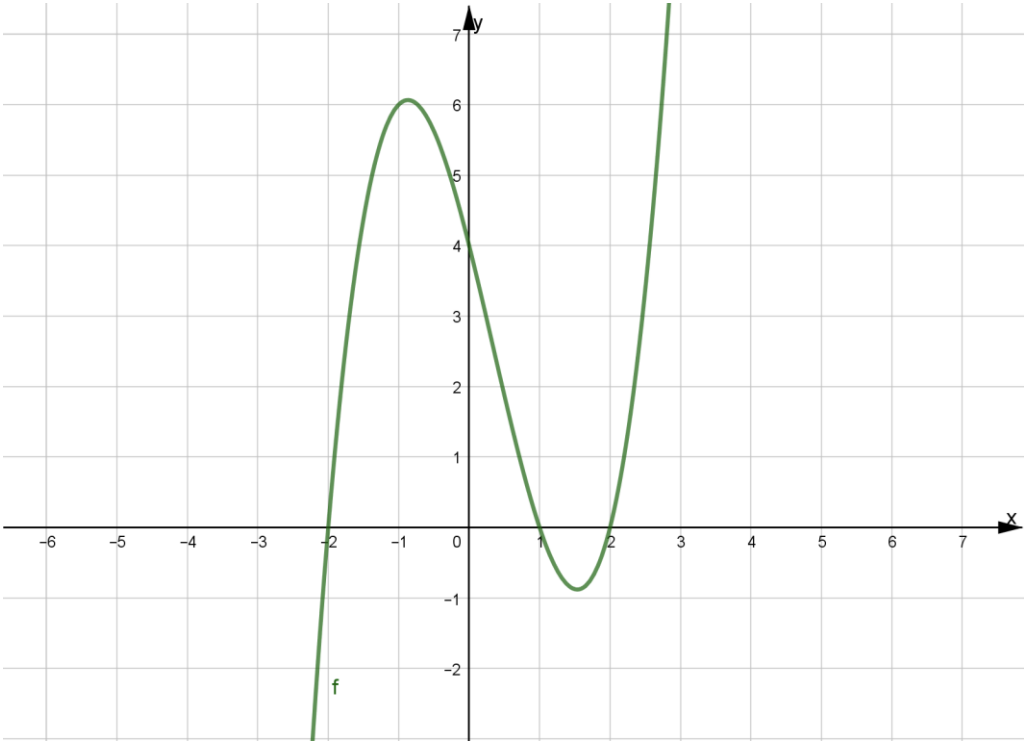
\includegraphics[scale=0.5]{mat16.1.png}
  \end{center}
  \caption{graf for $f$}
  \label{fig:1}
  \end{figure}
\sol \\ 
\textbf{a.} Da den geometriske betydning af $f(x)$ blot er y-værdien, kan følgende udledes ved aflæsning på de steder af grafen, hvor y-værdien er $0$.
\[
f(x)=0 \implies x=-2 \lor x=1 \lor x=2
\] 
\pagebreak
\begin{question}{}{}
  Grafen for et tredjegradspolynomium $f$ ses på \cref{fig:2} 
\begin{itemize}
  \item[a.] Løs ved hjælp af grafen ligningen $f'(x)=0$ 
\end{itemize}
\end{question}
\begin{figure}[h]
\begin{center}
  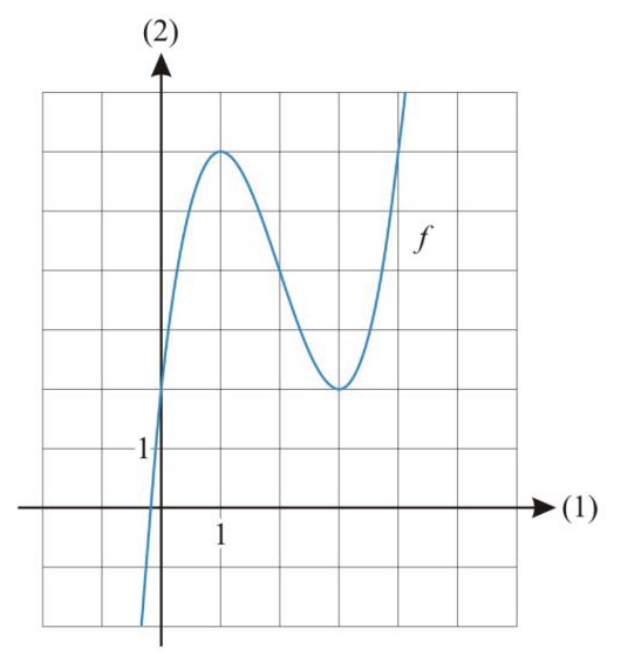
\includegraphics[scale=0.5]{mat16.2.png}
\end{center}
\caption{graf for $f$}
\label{fig:2}
\end{figure}
\sol \\ 
Ved toppunkterne af grafen er hældningen af tangenten$0$. Den geometriske betydning af $f'(x)$ er da hældningen af tangenten til grafen. Ved aflæsning må følgende gælde.
\[
f'(x)=0 \implies x=1 \lor x=3
\] 
\pagebreak
\begin{question}{}{}
  En del af grafen for $f$ er vist i \cref{fig:3}. Benyt den til at bestemme $f'(2)$.
\end{question}
\begin{figure}[h]
\begin{center}
  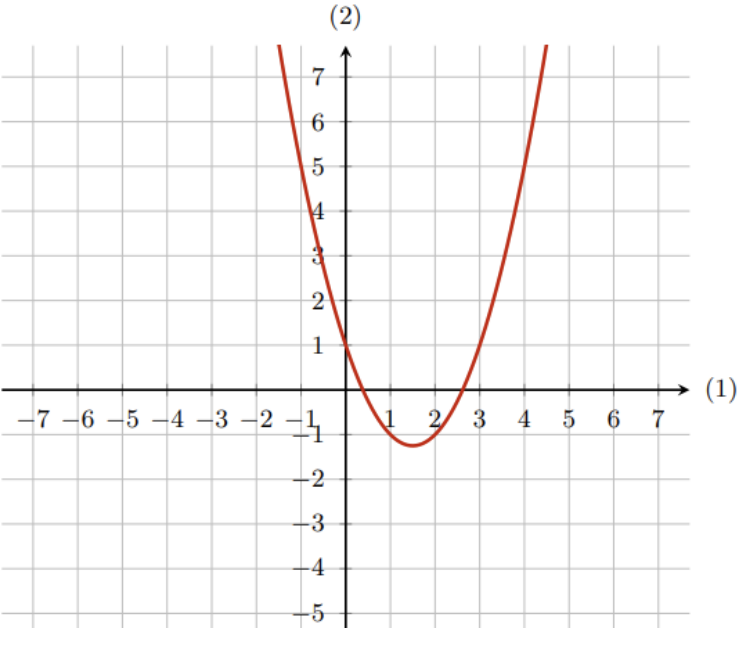
\includegraphics[scale=0.5]{mat16.3.png}
\end{center}
\caption{graf for $f$}
\label{fig:3}
\end{figure}
\sol\\ 
Lad $p$ denotere grafen for $f$. 
Det aflæses da på \cref{fig:3}, at $(0,1), (1,-1), (2,-1) \in g$. Siden grafen for $f$ er en parabel, er funktionsforskriften af formen $f(x)=ax^2+bx+c$. Vi kan nemt finde c-værdien med punktet $(0,1)$:
\[
(0,1)\in g \implies a\cdot 0+b\cdot 0+c=1 \iff c=1
\] 
Vi kan få lignende ud af de to andre punkter, hvor vi jo allerede kender c-værdien.
\begin{equation*}
\begin{split}
  (1,-1)\in g &\implies 1\cdot a+1\cdot b+1=-1\\ 
  (2,-1)\in g &\implies 2^2 \cdot a + 2\cdot b+1=-1
\end{split}
\end{equation*}
Vi har nu blot et simpelt ligningssystem, der skal løses.
\begin{equation*}
\begin{split}
  a+b+1=-1 \land 4a+2b+1=-1 &\implies b=-a-2 \land 4a+2b+1=-1\\ 
  &\implies 4a-2a-4+1=-1\\ 
  &\implies 2a=2\\ 
  &\implies a=1
\end{split}
\end{equation*}
b-værdien kan nemt regnes.
\[
b=-a-2=-1-2=-3
\] 
Da vi nu kender alle koefficienter og dermed funktionsforskriften, kan den afledede funktion findes.
\[
f(x)=x^2-3x+1 \implies \dv{x} (f(x))=2x-3
\] 
$f'(2)$ kan nu bestemmes:
\[
f'(2)=2\cdot 2-3=1
\] 

\begin{question}{}{}
  Bestem $\dv{f}{x}$ i hvert af følgende tilfælde:
\begin{itemize}
  \item[a.] $f(x)=3x+4$
  \item[b.] $f(x)=x^4+2x^3+4x$
  \item[c.] $f(x)=\ln(x)-4e^x+1$
  \item[d.] $f(x)=6\cdot \sqrt{x} + (x-1)^2$
  \item[e.] $f(x)=\frac{5}{x}-2x^{\frac{3}{2}}$
\end{itemize}
\end{question}
\sol \\ 
$f$ differentieres i alle delopgaverne:\\ 
\textbf{a.} 
\[
\dv{f}{x}=3
\] 
\textbf{b.}
\[
\dv{f}{x}=4x^3+3\cdot 2x^2+4=4x^3+6x^2+4
\] 
\textbf{c.}
\[
\dv{f}{x}=x^{-1} - 4e^x
\] 
\textbf{d.}
\[
\dv{f}{x}= 6\cdot \frac{\sqrt{x} }{2}+2x-2=3 \sqrt{x} +2x-2
\] 
\textbf{e.}
\[
\dv{f}{x} = -1\cdot 5x^{-2}-\frac{3}{2}\cdot 2x^{\frac{1}{2}}=- \frac{5}{x^2} - 3 \sqrt{x} 
\] 

\begin{question}{}{}
Definér $f:\mathbb{R} \to \mathbb{R}$ ved 
\[
  f(x)=3x^2-6x+5
\] 
Grafen for $f$ er en parabel. 
\begin{itemize}
  \item[a.] Bestem en ligning for tangenten til grafen for $f$ i punktet $P\left(2,f(2)\right)$ 
  \item[b.] Tegn i samme koordinatsystem grafen for $f$ og den fundne tangent fra sp. a.
\end{itemize}
\end{question}
\sol \\ 
\textbf{a.} I punktet $P\left(2,f(2)\right)$ er ligningen for tangenten da følgende, siden hældningen af linjen er differentialkvotienten for $f$  i 2, og konstantleddet blot er tangentens skæring med y-aksen.
\begin{equation*}
\begin{split}
  y&=f'(2)\cdot x + f(2) - f'(2)\cdot 2\\
  &= (6\cdot 2-6)\cdot x+5-(6\cdot 2-6)\cdot 2\\ 
  &=6x-7
\end{split}
\end{equation*}
\textbf{b.} I \cref{fig:4} ses grafen for $f$ og den fundne tangent tegnet i det samme koordinatsystem i GeoGebra.
\begin{figure}[h]
\begin{center}
  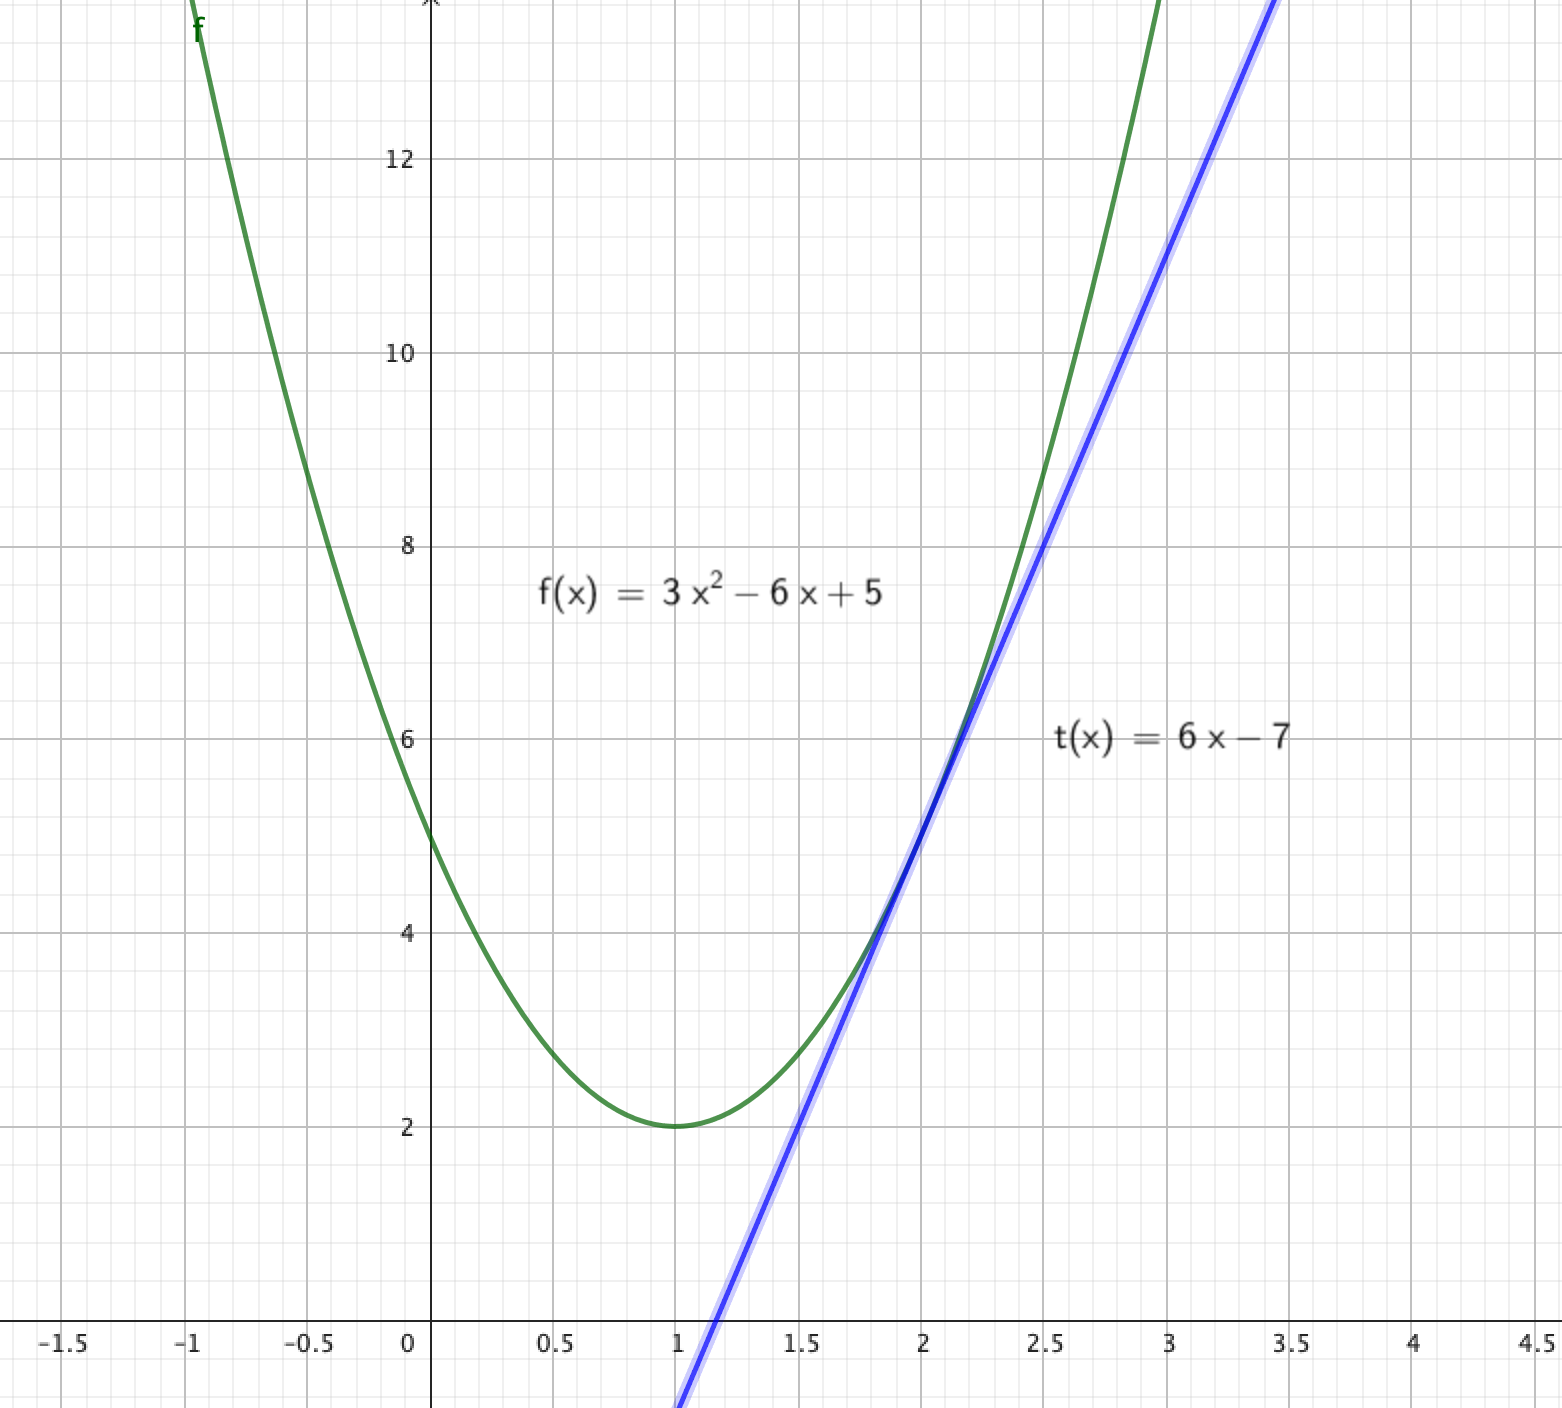
\includegraphics[scale=0.5]{Mat16_4.png}
\end{center}
\caption{Grafen for $f$ og den fundne tangent tegnet i GeoGebra }
\label{fig:4}
\end{figure}
\end{document}
